\chapter{Metodologia}
\label{chap:metodologia}

\section{Obtenção e Processamento dos Dados}
\label{sec:obtencao-processamento-dados}

Tanto para o processo de treinamento quanto para o processo de teste de uma RNA, o primeiro passo a ser dado é a obtenção das amostras experimentais para o treinamento supervisionado e teste das RNAs. Algoritmos de aprendizado máquinas supervisionadas são muito mais eficazes quando treinados com conjuntos de dados muito grandes.

Em 1 de dezembro de 2018, o aLIGO Scientific Collaboration e o Virgo Collaboration anunciaram o GWTC-1 \cite{Abbott_2019}, catálogo de GW observadas pelo aLIGO e Virgo durante a primeira e a segunda execução de observações, contendo os resultados completos de suas pesquisas por GW, que conta com onze detecções de GW provenientes dez de sistemas binários de buracos negros e um sistemas binário de estrelas de nêutrons.

O primeiro passo dado nesta pesquisa foi a coleta dos dados das GWs, as quais estão disponíveis no catálogo GWTC-1 através do Gravitational Wave Open Science Center (GWOSC)\footnote{\href{https://www.gw-openscience.org/about/}{ttps://www.gw-openscience.org/about/}}~\cite{vallisneri2015ligo}. Como as fusões de buracos negros dominam o número de detecções de GW, este trabalho focou exclusivamente neste tipo de detecção.

Após a obtenção dos dados, foram analisados e selecionados nove das dez amostras de GW de fusão de buracos negros, sendo elas: GW150914, GW151012, GW151226, GW170104, GW170608, GW170729, GW170809, GW170814, GW170823. As quais foram processadas com a ajuda da ferramenta PyCBC\footnote{\href{https://pycbc.org/}{https://pycbc.org/}}~\cite{alex_nitz_2019_2801307}, que é um pacote de software escrito em Python\footnote{\href{https://www.python.org/}{https://www.python.org/}}, usado para explorar e analisar as fontes astrofísicas de GW, e capaz de detectar binários compactos coalescentes e medir seus parâmetros astrofísicos. O PyCBC contém diversos módulos para processamento de sinais e um deles é capaz de gerar formas de GW. A partir desse módulo foi gerado uma forma de GW equivalente ao formato real das GW capturados pelos detectores de GW (Hanford-H1 e Livingston-L1 Interferômetros) para cada uma das amostras selecionadas.

Devido aos detectores terem uma alta sensibilidade, ruídos de origens instrumentais, ambientais e provenientes de atividades humanas sempre o atingem, poluindo os sinais e dificultando as detecções. Durante todo o processo os dados oriundos do aLIGO foram limpos e filtrados e também ignoradas as falhas, os blips e outras fontes de ruído de detectores transientes que dificultam a analise e processamento das GW.

As formas de GW são geradas como uma série temporal, usando uma das aproximações de forma de onda disponíveis pelo PyCBC. Os parâmetros principais foram as massas do sistema binário (dadas em massas solares), o tempo entre as amostras (em segundos), a frequência inicial das GW (Hz) e o nome do aproximante que gostaríamos de gerar. Está disponível uma variedade de aproximações que incluem diferentes efeitos físicos. A precisão numérica depende da resolução, enquanto a precisão da extrapolação pode ser avaliada pela comparação de diferentes ordens de extrapolação. Pedidos mais altos tendem a produzir melhores resultados na fase inspiral, mas pior na fase do ringdown \cite{scharpf2017simulation}. 

Desta forma optou-se por buscar aproximadores com níveis mais elevados de precisão que tivessem o melhor resultado para ambas as fases das simulações, devido a resultados mais atualizados e mais precisos. Para esta pesquisa foi usado o aproximante IMRPhenomD, pois atende altos níveis de precisão graças a uma combinação de métodos analíticos \textit{post-Newtonian} (PN) e \textit{effective-one-body} (EOB) para descrever a inspiração, e a calibração de modelos fenomenológicos de fusão-ringdown para simulações de relatividade numérica (NR)~\cite{khan2015frequencydomain}. Ele modela a forma de GW nas fases de inspiração, fusão e ringdown dos buracos negros e inclui a capacidade de cada buraco negro girar na mesma direção que a órbita (rotação alinhada), atingindo bons resultados em ambas as fases de inspiral e ringdown. Além de poderem ser geradas rapidamente e para uma ampla gama de valores de parâmetros.

O PyCBC foi usado no projeto descrito nesta tese tanto para geração de banco de modelos quanto todo o processo de filtragem correspondente dos dados brutos advindos do aLIGO. Usamos o PyCBC para geração simples de GW no domínio da frequência com massas e tempo de amostras iguais as dos sistemas binários descritos no catalogo GWTC-1 com uma frequência inicial de 20Hz. Portanto, foram gerados dezoito GW equivalentes as GW detectadas pelo aLIGO, nove para cada detector aLIGO (Hanford-H1 e Livingston-L1).

A escolha e adequação dos dados utilizados para treinar e testar uma RNA é de fundamental importância. É necessário que se disponha de dados em quantidade e qualidade suficientes. Caso a quantidade de dados seja pequena, a rede não conseguirá criar um modelo suficientemente representativo para se ter um desempenho satisfatório quando aplicado em situações reais após o seu desenvolvimento, o que é chamado de sobre-ajuste (overfitting) dos dados. Além disto, os dados devem englobar todos os aspectos do problema em questão, a fim de que o modelo criado seja genérico. 

Como o objetivo é treinar uma RNA que forneça um diagnóstico classificativo entre GW e Ruído, que apresente um bom desempenho, extraímos um intervalo de 0.1 segundos de cada forma de onda com pico centralizado, deslocando a localização de pico de cada sinal aleatoriamente dentro de um intervalo de 0 a 0.05 segundos para a direita, a uma taxa de amostragem de 4096Hz. Este processo foi repetido 600 vezes para cada uma das formas de onda geradas, criando assim 10800 modelos de GW, a Figura~\ref{fig:gw150914-offset} ilustra algumas das ondas geradas.

\begin{figure}[ht]
    \centerline{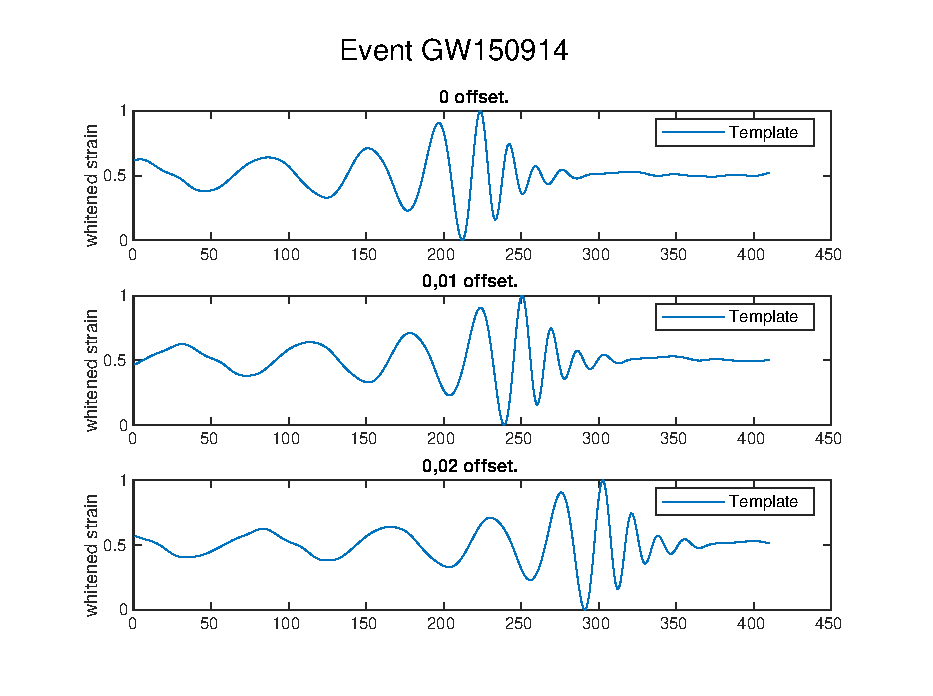
\includegraphics[width=1\textwidth]{figuras/GW150914.eps}}
    \caption{Alguns modelos de GW com deslocamento}
    \label{fig:gw150914-offset}
\end{figure}

Os modelos de machine learning são construídos para minimizar erros. Desde que a probabilidade pertence a classe com maior número de observação, o algoritmo estará enviesado em classificar as novas observações. Afim de evitar o enviesamento por causa do desbalanceamento dos dados, foi criado também a mesma quantidade de amostras de ruído com espectro equivalente a densidade espectral de potência (DEP ou PSD em inglês) do ruido do aLIGO~\cite{T1800044}. No final da construção dos dados, juntamos os dois bancos de dados (ruídos e ondas), totalizando o conjunto de dados de treinamento, teste e validação com um total de 21600 amostras com duas classes: Ondas e Ruídos.

É esperado que uma RNA, após a fase de treinamento, seja capaz de produzir respostas corretas a estímulos externos, mesmo que estes não sejam exatamente iguais aos estímulos utilizados no seu treinamento. Para o conjunto de dados de novos estímulos, foram necessários 2.0 segundos de observação a uma taxa amostral de 4096Hz de cada um das nove GW selecionadas anteriormente, filtradas com a onda centralizada, na qual eles foram separados em várias janelas de 0.1 segundos (410 pontos) com passos de uma unidade e a mesma taxa de frequência amostral, gerando assim aproximadamente ~7780 janelas de dados. Esses dados foram gerados para os dois detectores aLIGO (Hanford-H1 e Livingston-L1) separadamente, totalizando aproximadamente ~140000 de dados.

Alguns algoritmos têm dificuldade em entender variáveis que têm mais do que uma categoria. Pelo fato dos dados apresentarem duas classes categóricas (onda e ruído) o algoritmo de Machine Learning que empregamos nesta pesquisa não produz bons resultados com esses dados categóricos. Diante dessa limitação foi preciso converter as variáveis categóricas para valores numéricos. Buscando melhorar o processamento dos dados foi aplicado uma técnica de pré-processamento de dados chamada one-hot encoding. 

O one-hot encoding é usada em Machine Learning como um método para quantificar dados categóricos e melhorar significativamente os resultados \cite{sarkar2017practical}. Em resumo, esse método produz um vetor com comprimento igual ao número de categorias no conjunto de dados. Neste caso, as classes onda e ruído são transformadas em vetores como: $[1,0]$ e $[0,1]$ respectivamente, que indicam a saída correspondente desejada da RNA para cada uma das classes do conjunto de dados.

Com essa imensa quantidade de dados seria difícil manter tudo sobre estruturas de arquivos simples separados por vírgulas (CSV do inglês comma-separated-values), pois além de consumir muito espaço físico o processo de leitura desses arquivos se tornaria demasiadamente longo. Para resolver este problema, todos os conjuntos de dados foram salvos em HDF (Hierarchical Data Format), que é uma biblioteca de software e formato de dados de alto desempenho (HDF4, HDF5) projetados para armazenar e organizar grandes quantidades de dados para facilitar a leitura dessa grande massa de dados~\cite{hdf}. Por usar árvores B para indexar os dados, o HDF funciona bem para dados de séries temporais. A maior parte dos dados entra em matrizes simples que podem ser acessadas muito mais rapidamente do que as linhas de um banco de dados SQL. 

O HDF foi desenvolvido para processamento e armazenamento de E/S rápidos de alto desempenho com um rico conjunto de recursos de desempenho integrados que permitem otimizações de tempo de acesso e espaço de armazenamento~\cite{hdf}. Esta biblioteca foi amplamente adotada em vários setores e é o padrão de fato na comunidade científica e de pesquisa, uma vez que a maioria das ferramentas que usa Machine Learning suportam esse tipo de arquivo.

\section{Arquitetura da Rede Neural}
\label{sec:arquitetura-rna}

Definir a arquitetura de uma RNA é muito importante devido ao fato de que seu arranjo depende do problema a ser tratado. Ademais, a arquitetura da rede está diretamente relacionada ao algoritmo de aprendizagem usado para treinamento. De acordo com o teorema da aproximação universal, aplicado às redes MLP, uma única camada escondida de neurônios é suficiente para realizar uma aproximação de qualquer função contínua para um dado conjunto de treinamento representado pelo conjunto de entradas e a saídas-alvo \cite{cybenko1989approximation, haykin2007redes}.

Com base nesta premissa, foi desenvolvida uma arquitetura de RNA simples para otimizar e acelerar o processo de treinamento e detecção de GWs. Foi gasto um tempo significativo pesquisando por tentativa e erro uma ótima arquitetura de RNA e otimizando hiperparâmetros. Após sucessivas simulações para determinação do número de entradas das redes neurais, foi estabelecido que a rede neural teria 410 entradas. Sendo assim, cada janela de dados das GW seria apresentados à rede, ou seja, o classificador será aplicado ao fluxo de dados contínuo usando janelas deslizantes de 0,1 segundo de largura com uma diferença de 200 microssegundos.

Diversas estruturas de RNA do tipo MLP com diferentes quantidades de neurônios na camada oculta e diferentes funções de ativação foram testadas visando obter a melhor e mais otimizada estrutura MLP a ser empregada nesta dissertação para a detecção de GWs. Decidir o número de neurônios na camada oculta é um aspecto complexo e um fator que afeta o desempenho das redes treinadas. Segundo \cite{OKOH201619}, a prática mais plausível é treinar várias redes que variam o número de neurônios da camada oculta e, em seguida, selecionar a melhor delas usando um índice de desempenho.

No entanto, foi possível aprimorar ainda mais a discriminação da RNA graças a implementação do \textit{one-hot encoding}, que é um processo pelo qual variáveis categóricas são convertidas em um formato binário que pode ser fornecido aos algoritmos de RNA para fazer um trabalho melhor na classificação \cite{buckman2018thermometer}. Com essa técnica foi possível definir duas categorias quantizadas representadas pelos valores binários de 0 e 1, consequentemente a RNA acompanhou a quantidade de saída desejada e foi colocado duas saídas na última camada da RNA, as saídas A e B. 

Agora, por exemplo, se o estimulo de entrada da rede fosse da classe ``Onda'', as saídas da RNA desejadas seriam A = 1 e B = 0 [1,0] e se o estimulo de entrada fosse da classe ``Ruído'', as saídas da RNA desejadas seriam A = 0 e B = 1 [0,1]. Com essas duas saídas, é possível definir um score como:

\begin{equation}
score = \frac{a-b}{2}+0.5
\label{eq:score}
\end{equation}

Dessa forma, a saída da RNA desejada para a classe Onda terá uma pontuação que tenderá a 1 ($score \rightarrow 1$), e a saída da RNA desejada para a classe Ruído terá uma pontuação que tenderá a 0 ($score \rightarrow 0$). 

Durante o processo de encontrar a melhor estrutura e parâmetros para a rede, o modelo foi avaliado através de uma análise de distribuição dos resultados, do erro quadrático médio (MSE) e do cálculo da estatística de Kolmogorov-Smirnov (KS). Graças ao score desenvolvido na Equação \ref{eq:score}, foi possível construir uma distribuição de pontuação para cada classe, e a capacidade de discriminação da RNA pode ser medida com o uso da distância KS. Essa distância KS é a distância máxima entre duas funções de Distribuição Empírica Acumulada (ECD do inglês \textit{Empirical cumulative distribution}), que quando normalizadas são um valor na faixa [0,1]. O KS é descrito pela teoria estatística não paramétrica e é utilizada para testar se as distribuições de dois grupos são iguais~\cite{daniel2000applied}. 

O teste de KS tem sido utilizado para avaliar o desempenho de classificadores binários avaliando a diferença entre as distribuições dos maus e bons clientes \cite{karcher2009redes} e distribuição do cliente mais propensos a quitar suas dividas ou não \cite{forti2018tecnicas}  por exemplo, neste caso, quanto maior for a estatística de KS, maior será a separação entre os clientes adimplentes e inadimplentes como também entre cliente quitados e não quitados respectivamente. 

Em outras palavras, para esta pesquisa ele avalia o quão bem o modelo consegue distinguir os classificados como Onda dos classificados como Ruído. Sendo assim, o KS se comporta como uma medida de avaliação de performance, quanto maior for o resultado do KS (indicação de maior diferença entre as distribuições), melhor está a acurácia do modelo, pois a separação das classes é maior. 

A estatística de Kolmogorov–Smirnov pode ser descrita por: 
\begin{equation}
KS = Max|F1(x)−F2(x)|
\label{eq:kolmogorov}
\end{equation}
onde $Max$ é a maior distância entre as distribuições de $F1$ e $F2$, em que, $F1$ é a distribuição acumulada do score dos classificados como Ondas e $F2$ é a distribuição acumulada do score dos classificados como Ruído.

É mostrado na Figura~\ref{fig:ANN_Distribution_a} uma ilustração pictórica da distribuição empírica do score gerado para o problema de classificação binária, onde a classe $X$ tem uma distribuição do score centrada em torno de $0$ e a classe $Y$ tem uma distribuição do score em torno de $1$. É mostrado na Figura~\ref{fig:ANN_Distribution_b} a distância KS entre essas duas distribuições.

\begin{figure}[H]
\centering
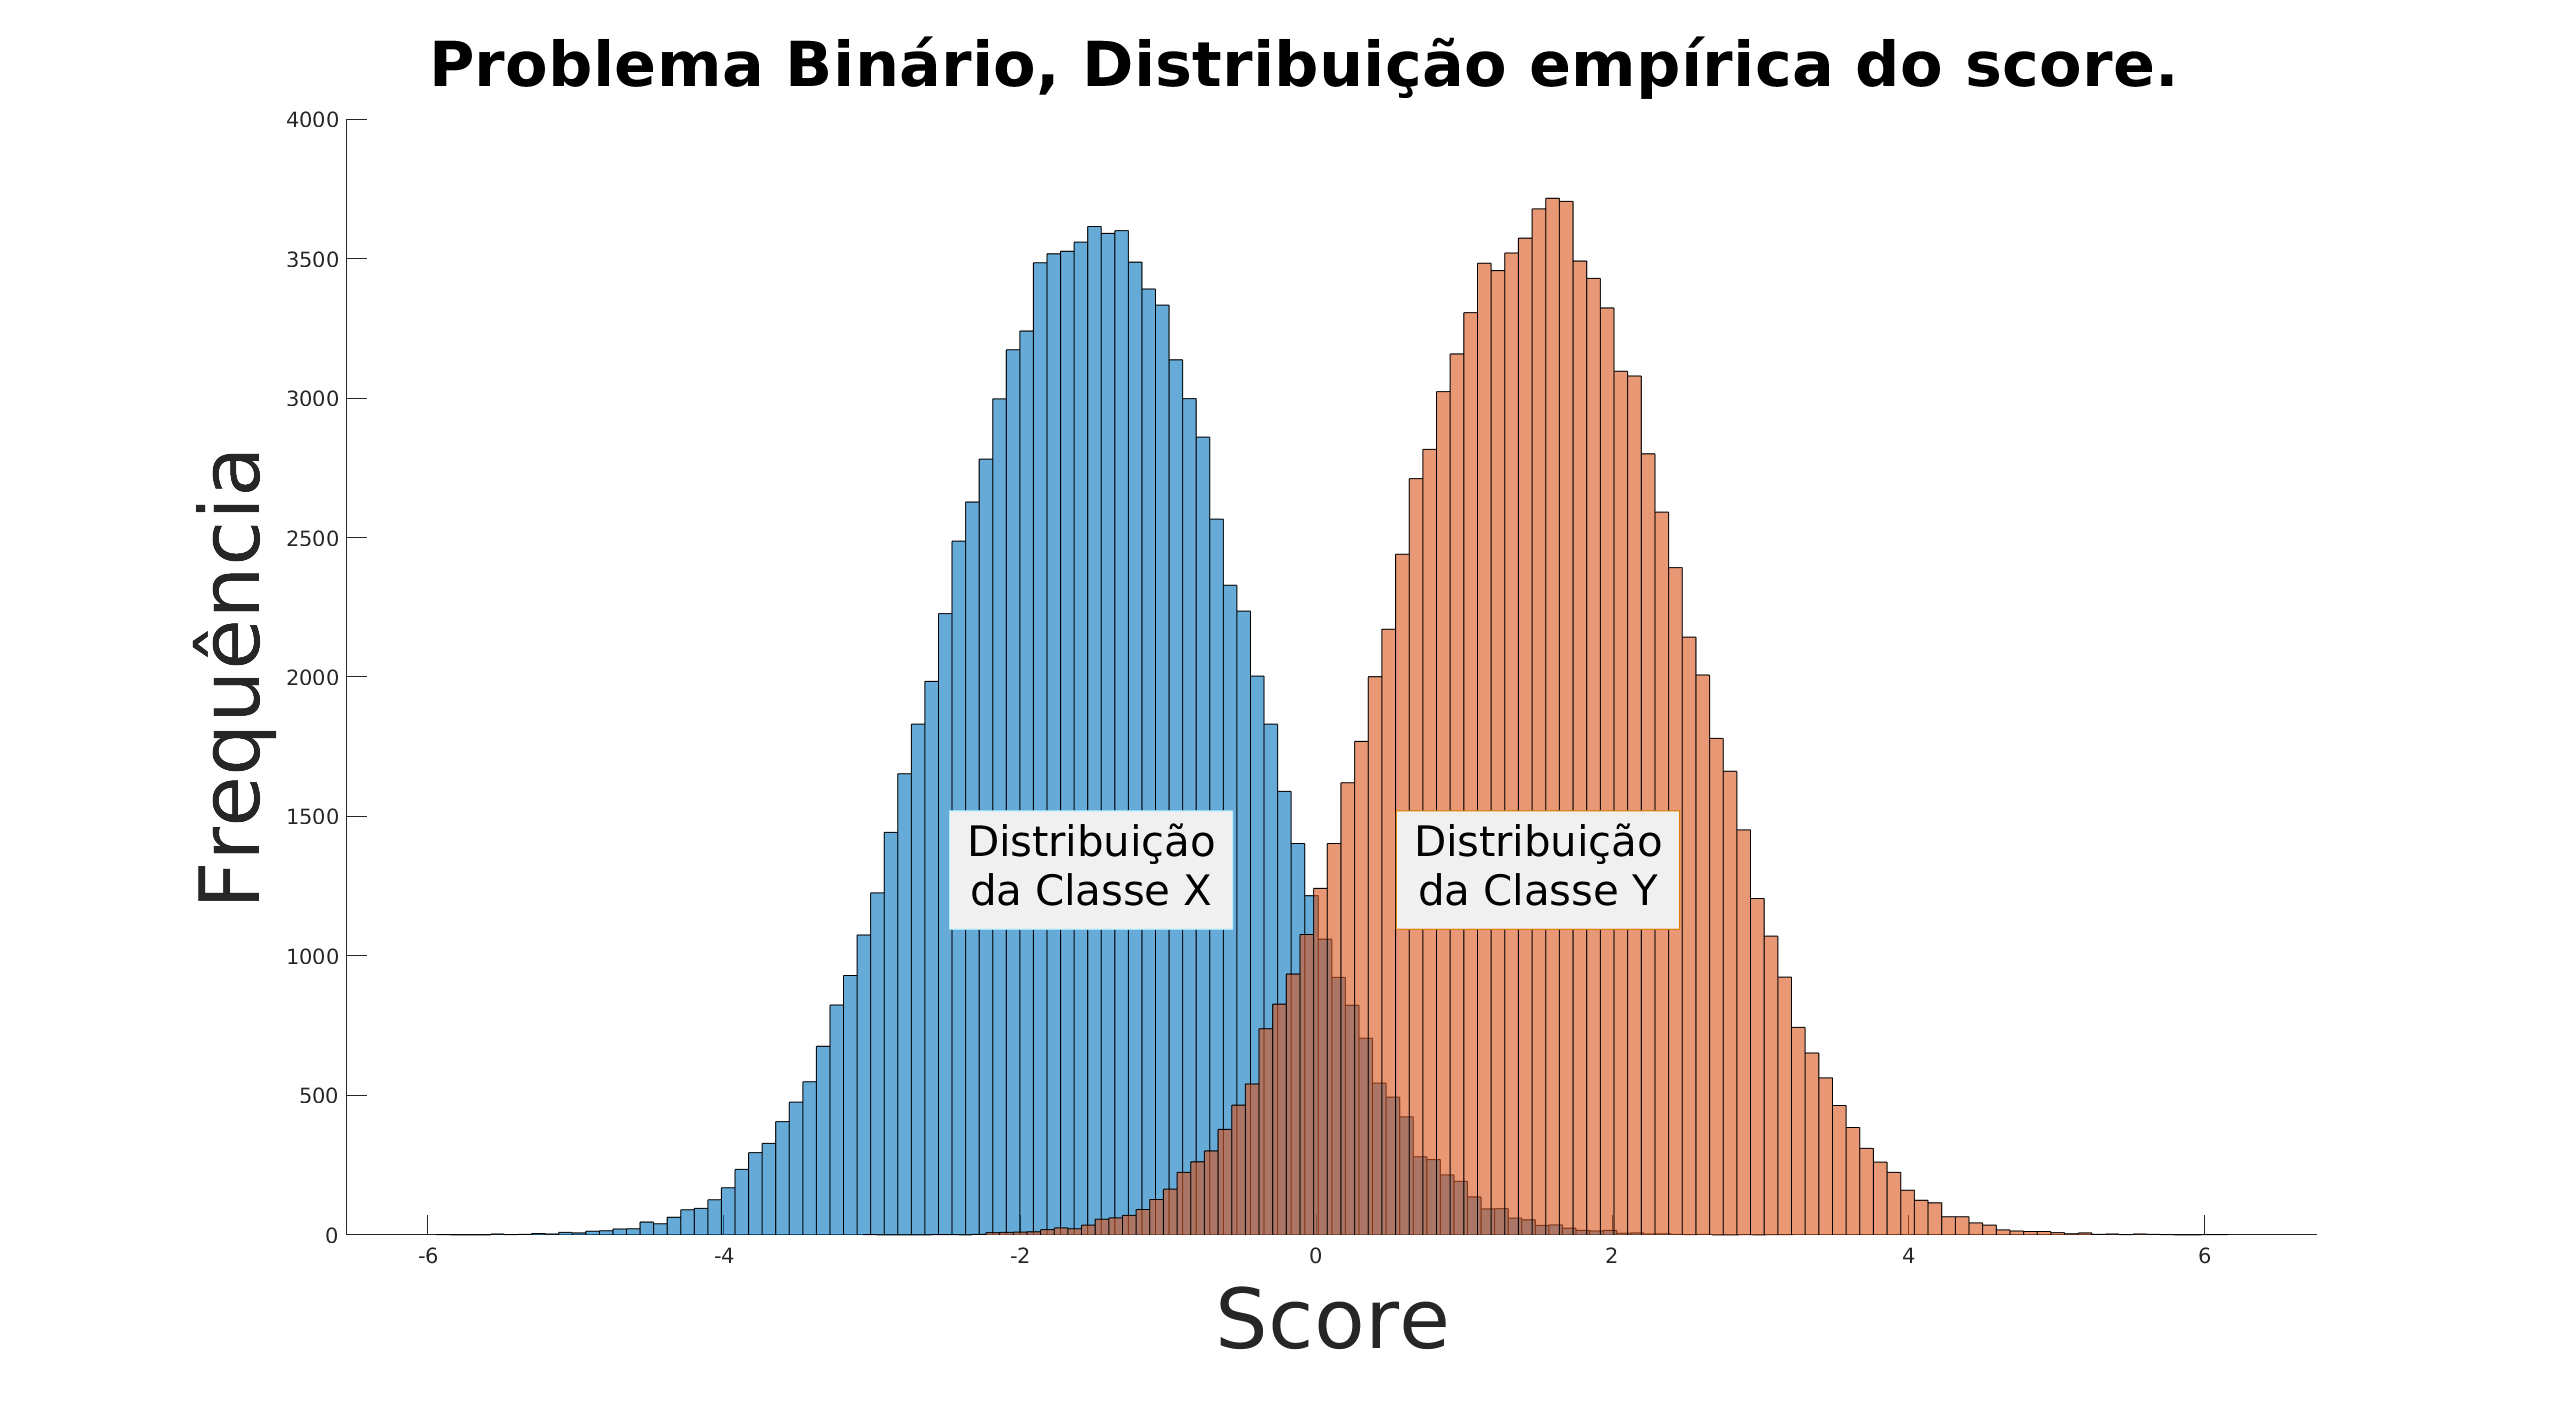
\includegraphics[width=1\textwidth]{figuras/hitograma_distribuicao_empirica_score.eps}
\caption{Resposta pictórica do score da RNA para um problema de classificação binária - Distribuição empírica do score.}
\label{fig:ANN_Distribution_a}
\end{figure}

\begin{figure}[H]
\centering
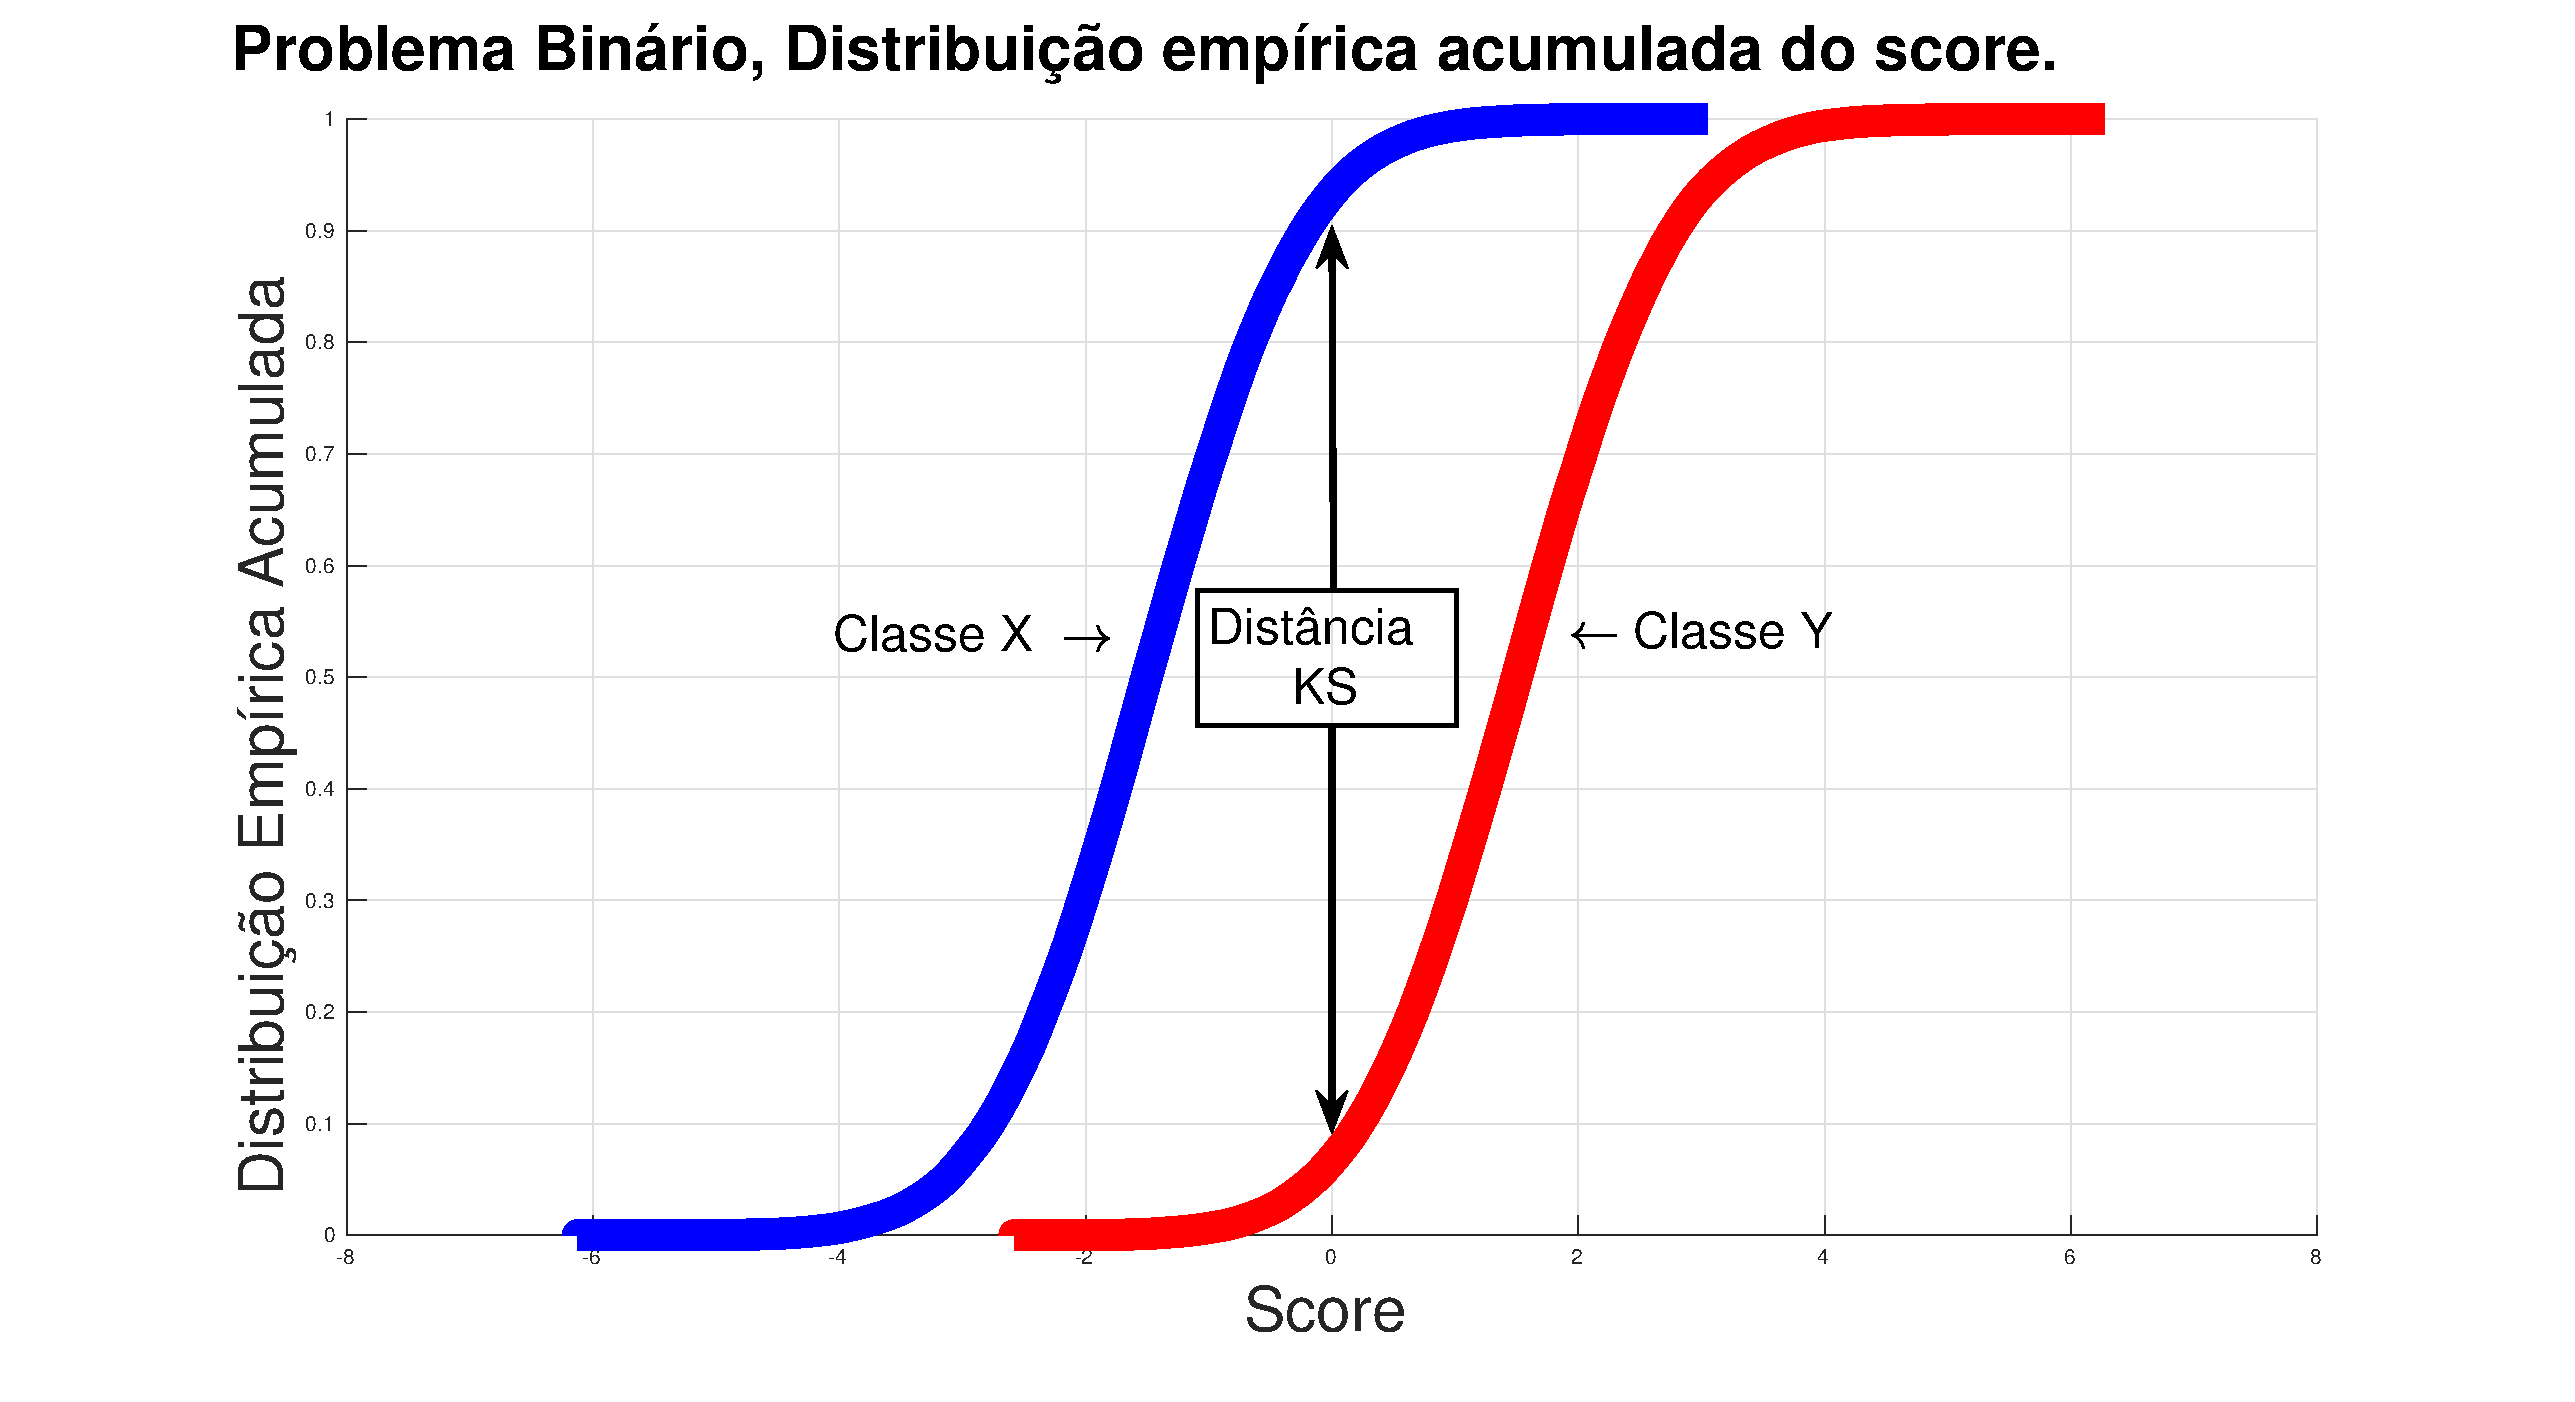
\includegraphics[width=1\textwidth]{figuras/distribuicao_empirica_acumulada_score.eps}
\caption{Resposta pictórica do score da RNA para um problema de classificação binária --- Distribuição empírica acumulada do score.}
\label{fig:ANN_Distribution_b}
\end{figure}

\section{Treinamento da Rede}
\label{sec:treino-rna}

O principal objetivo do processo de aprendizagem de uma RNA é fazer com que um conjunto de entradas produza um conjunto de saídas desejadas ou, no mínimo, um conjunto de saídas aceitável, ao serem aplicadas em uma RNA~\cite{haykin2007redes}.

Para uma RNA, o conceito de treinamento se diferencia do conceito de aprendizado. O aprendizado está associado a uma tarefa que a rede está executando em função do treinamento e da sua modelagem. Já o treinamento é o processo de ensinar a RNA~\cite{furtado2019redes}.

Pode-se dizer que o treinamento da rede neural é o ponto mais critico que determina o desfecho da rede, pois, neste procedimento, a rede é submetida ao aprendizado, onde alguns fatores dos parâmetros de treinamento são relevantes, como: o algoritmo de treinamento, o número máximo de iterações, a taxa de aprendizagem, a função de ativação e muitos outros.

A seleção dos parâmetros de treinamento de uma RNA pode ser um processo complexo, pois pequenas diferenças nestes parâmetros podem levar a grandes diferenças tanto no tempo de treinamento como na generalização obtida.

Nesta pesquisa foram testados diversos algoritmos de aprendizagem, tanto de primeira ordem como de segunda ordem, como RProP, Gradiente Conjugado, Quase-Newton e Levenberg–Marquardt. Contudo, o algoritmo de Backpropagation com taxa de aprendizado adaptativa encontrou os melhores resultados, embora não tenha sido o mais rápido computacionalmente. Para sua utilização, alguns parâmetros inerentes do algoritmo precisaram ser definidos, como: taxa de aprendizagem $\eta$ entre $0.5$ e $0.9$, exceto nos casos de taxa adaptativa, O numero de épocas foi definido com $100000$ épocas.

As funções de ativação são um elemento de extremamente importante das RNAs. Elas basicamente decidem se um neurônio deve ser ativado ou não. Ou seja, se a informação que o neurônio está recebendo é relevante e deve ser propagada ou não~\cite{DeepLearningBook}. Para que se encontrasse a função de ativação que melhor se adequasse as redes desenvolvidas nesta pesquisa, foram usadas somente três funções de ativação, são elas: Linear, Sigmoide e Tangente Hiperbólica.

Uma das dificuldades do processo de treinamento de uma RNA consiste em encontrar o melhor ponto de parada do treinamento, pois o erro de treinamento começa com um valor muito alto, decai rapidamente, e continua diminuindo lentamente, tendendo a atingir um mínimo local na superfície de erro~\cite{haykin2007redes}. Para isto, existem vários métodos para a determinação do momento em que o treinamento de uma RNA deve ser encerrado. Uma boa determinação deste momento é fundamental para um bom treinamento e consequentemente uma boa generalização. Portanto, o treinamento é interrompido quando a rede apresenta uma boa capacidade de generalização e quando a taxa de erro é pequena, menor que um erro aceitável. É necessário encontrar um ponto ótimo de parada com o menor erro possível e capacidade de generalização máxima~\cite{barros2018avaliaccao}.

Neste sentido, o critério de parada no processo de treinamento foi o número máximo de iterações de $100000$ épocas, taxa de erro médio por época de $1e^{-15}$ e sua capacidade de generalização com $100$ validações. Desta forma, o treinamento é encerrado quando qualquer um dos critérios é atendido.

Em relação aos pesos sinápticos, eles foram inicializados com números randômicos, mantendo o cuidado de não serem grandes suficientes para saturarem os neurônios, nem pequenos a ponto de atrasarem o aprendizado.

Para o conjunto de dados, normalmente são separados em dois conjuntos: conjunto de treinamento, que é usado para treinar a rede e conjunto de teste, que é utilizado para verificar a performance da rede sob condições reais de utilização. 

Afim de evitar o problema de overfitting, foi feita um subdivisão do conjunto de treinamento, criando um conjunto de validação, usado para verificar a eficiência da rede quanto a sua capacidade de generalização durante o processo de treinamento, o que se justifica o seu uso como critério de parada do treinamento da rede.

O conjunto de total de dados contém exatos 21600 amostras de dados, separados em duas classes igualmente. Desses dados, 70\% são para treinamento, 15\% para validação e 15\% para teste. O conjunto de dados reais para execução contém aproximadamente ~140.000 padrões de entrada, que são usados para a resolução final da rede executando situações reais com a rede treinada.

Depois de determinar estes conjuntos, eles foram colocados em ordem aleatória para prevenção de tendências associadas à ordem de apresentação dos dados. Além disso, todos os valores de entrada foram normalizados no intervalo [0,1].

\section{Construção do Comitê}
\label{sec:comite}

A grande disponibilidade de recursos computacionais, possibilitou a criação de múltiplas propostas de soluções, as quais foram descartadas como testes e ajustes dos parâmetros para a busca do melhor modelo (rede). Entretanto, visto que, em certo ponto da pesquisa as RNAs descartadas apresentavam um desempenho parecido e com resultados consistentes, foi possível implementar um comitê de redes neurais.

De acordo com \cite{haykin2011neural}, a combinação do conhecimento adquirido pelas RNAs para chegar a uma solução global é supostamente superior àquela obtida por qualquer RNA única. Sendo assim, várias RNAs com a melhor configuração foram treinadas e dentre elas foram selecionadas 500 modelos com o melhor desempenho que formaram a máquina de comitê de redes neurais.

A máquina do comitê desenvolvida na Figura~\ref{fig:comite} mostra um número k, em que k = 500 RNAs treinadas individualmente de maneira independente que compartilham uma entrada comum e cuja saída individual é combinada para produzir uma saída geral. As saídas dessas redes são colocadas em um módulo de combinação que executa a função de calcular a média das saídas combinadas de todas as RNAs do comitê e apresentar o resultado do comitê de RNA.

\begin{figure}[H]
\centering
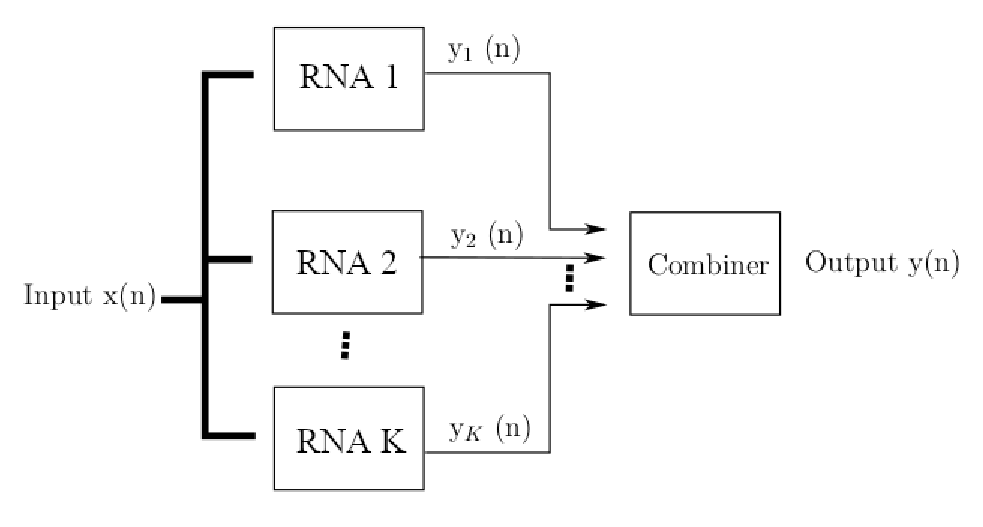
\includegraphics[width=1\textwidth]{figuras/comite.eps}
\caption{Diagrama de blocos de uma máquina de comitê.}
\label{fig:comite}
\end{figure}

Para implementação, execução e teste das RNAs, o software Matlab® R2018b\footnote{\href{ https://www.mathworks.com/products/matlab.html} {https://www.mathworks.com/products/matlab.html}} foi escolhido. Por possuir uma interface gráfica de treinamento de redes neurais, esse aplicativo suporta os mais diversos tipos de algoritmos de treinamento de redes neurais, permitindo que se possa executar uma extensa árvore de testes na tentativa de definir o modelo neural mais adequado, além de seu amplo uso pela comunidade científica.